\begin{definition}[Suporte]
  Seja $f:X\subseteq\mathbb{R}^{n}\to\mathbb{R}$ uma função.\\
  Definimos  \textbf{suporte} de $f$ como sendo
  \begin{align*}
    \supp f=\{x\in X:f(x)\neq 0\}.
  \end{align*}
  Dizemos que $f$ tem suporte compacto se $\supp f$ é compacto. 
\end{definition}
\begin{definition}[Extensão contínua]
  Sejam $U\subseteq\mathbb{R}^{n}$ aberto e $f:U\to\mathbb{R}$ uma função contínua com suporte compacto. Definimos a \textbf{extensão contínua} de $f$ dada por
  \begin{align*}
    \tilde{f}:\mathbb{R}^{n}&\to\mathbb{R},\\
                           x&\to \begin{cases}
                             f(x), &\text{ se } x\in U \text{,} \\
                            0, &\text{ se } x\notin U.
                           \end{cases}
  \end{align*}
\end{definition}
Note que se $A$ é um bloco que contém $U$, definimos
\begin{align*}
  \int_{U}f(x)\,dx=\int_{\mathbb{R}^{n}}\tilde{f}(x)\,dx.
\end{align*}
\begin{definition}[Bumb function]
  Definimos $\phi:\mathbb{R}^{n}\to\mathbb{R}$ como a \textbf{bumb function} dada por
  \begin{align*}
    \phi(x)=\begin{cases}
      e\cdot e^{-\frac{1}{1-|x|^{2}}}, &\text{ se } |x|<1 \text{,} \\
      0, &\text{ se } |x|\geq 1.
    \end{cases}
  \end{align*}
  \begin{center}
    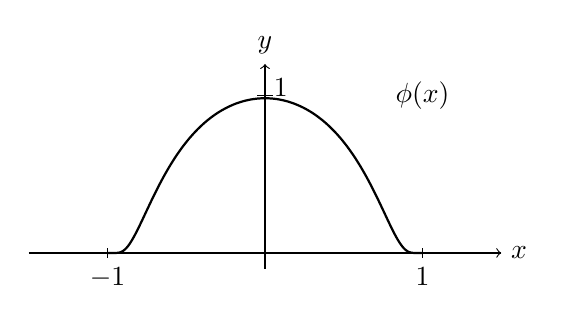
\begin{tikzpicture}[scale=2]

  % Ejes
  \draw[->] (-1.5,0) -- (1.5,0) node[right] {$x$};
  \draw[->] (0,-0.1) -- (0,1.2) node[above] {$y$};

  % Bump function
  \draw[
      domain=-0.999:0.999,
      samples=200,
      smooth,
      thick
  ]
  plot (\x,{2.67*exp(-1/(1-\x*\x))});
  
  % Parte cero
  \draw[thick] (-1.5,0) -- (-1,0);
  \draw[thick] (1,0) -- (1.5,0);
  
  % Marcas
  \draw (-1,0.03) -- (-1,-0.03) node[below] {$-1$};
  \draw (1,0.03) -- (1,-0.03) node[below] {$1$};
  \draw (-0.05,1) -- (0.05,1);
  \node at (0.1,1.05) {$1$};

  \node at (1,1) {$\phi(x)$};
\end{tikzpicture}

  
  \end{center}
  Note que $\phi\in C^{\infty}$ e $\supp \phi=\{x:|x|<1\}$.
\end{definition}
\begin{example}\label{ex:bumb-function}
  A bumb function pode ser utilizada para construir funções suaves com suporte compacto.
  \begin{align*}
    f(x)=\begin{cases}
      2, &\text{ se } |x|\leq 1,\\
      2\phi(x-1), &\text{ se } 1<x<2,\\
      2\phi(x+1), &\text{ se } -2<x<-1,\\
      0, &\text{ se } |x|\geq 2.
    \end{cases}
  \end{align*}
  Assim, $f$ é igual a $2$ no intervalo $[-1,1]$ e decai suavemente até $0$ fora desse intervalo.
  \begin{center}
    \begin{tikzpicture}[scale=1.2]

  % Eixos
  \draw[->] (-3,0) -- (3,0) node[right] {$x$};
  \draw[->] (0,-0.2) -- (0,2.5) node[above] {$f(x)$};

  % Parte constante
  \draw[thick] (-1,2) -- (1,2);

  % Decaimento suave à direita
  \draw[
    domain=1.001:1.999,
    samples=150,
    smooth,
    thick
  ]
  plot (\x,{2*exp(1)*exp(-1/(1-(\x-1)^2))});

  % Decaimento suave à esquerda
  \draw[
    domain=-1.999:-1.001,
    samples=150,
    smooth,
    thick
  ]
  plot (\x,{2*exp(1)*exp(-1/(1-(\x+1)^2))});

  % Parte zero
  \draw[thick] (-3,0) -- (-2,0);
  \draw[thick] (2,0) -- (3,0);

  % Linhas auxiliares
  \draw[dashed] (-1,0) -- (-1,2);
  \draw[dashed] (1,0) -- (1,2);

  % Marcas
  \draw (-2,0.05) -- (-2,-0.05) node[below] {$-2$};
  \draw (-1,0.05) -- (-1,-0.05) node[below] {$-1$};
  \draw (1,0.05) -- (1,-0.05) node[below] {$1$};
  \draw (2,0.05) -- (2,-0.05) node[below] {$2$};

  \draw (0,2.03) -- (-0.05,2.03);
  \node at (0.2,2.15) {$2$};

\end{tikzpicture}

  \end{center}
\end{example}
\begin{definition}[Cobertura localmente finita]
  Dizemos que uma cobertura de $X\subseteq\mathbb{R}^{n}$ é \textbf{localmente finita} se todo ponto $x\in X$ tem uma vizinhançã aberta que intersecta no máximo um número finito de conjuntos da cobertura. 
\end{definition}
\begin{definition}[Partição da unidade subordinada]
  Sejam $X\subseteq \mathbb{R}^{n}$ um conjunto arbitrário e $C=\{U_{\alpha}\}_{\alpha\in\mathcal{A}}$ a cobertura aberta de $X$.\\
  Uma partição da unidade subordinada $C$ é uma coleção $\{\rho_{\alpha}\}_{\alpha\in\mathcal{A}}$ de funções $C^{\infty}(\mathbb{R}^{n})$ tais que
  \begin{enumerate}[i)]
    \item $0\leq\rho_{\alpha}\leq 1$.
    \item $\supp(\rho_{\alpha})\subseteq U_{\alpha}$.
    \item $\{\supp(\rho_{\alpha})\}_{\alpha\in\mathcal{A}}$ é localmente finita.
    \item $\sum_{\alpha\in\mathcal{A}}\rho_{\alpha}=1$.
  \end{enumerate}
\end{definition}
\begin{note}
  Uma maneira de construir essas funções $\rho_{\alpha}$ é usando modificações da bumb function.
\end{note}
\begin{example}
  Seja $X=\mathbb{R}$ e seja $C=\{U_{k}\}_{k\in\mathbb{Z}^{+}}$ com $U_k=(-2+3k,2+3k)$ a cobertura aberta de $\mathbb{R}$, note que tomando $f$ como no exemplo \ref{ex:bumb-function}, definimos $f_k(x)=f(x-3k)$, logo $\{f_k\}_{k\in\mathbb{Z}^{+}}$ é uma partição da unidade subordinada a $C$.
  \begin{center}
      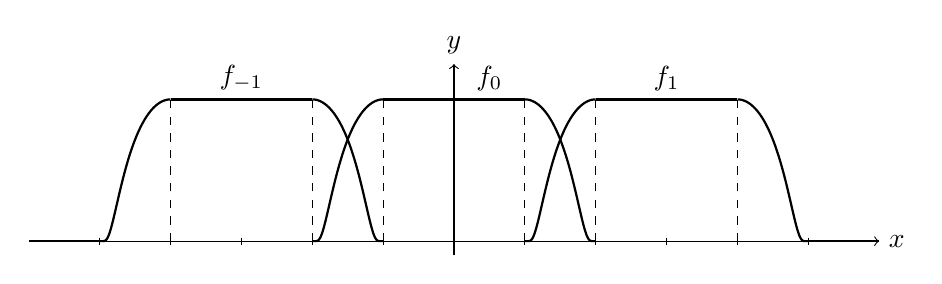
\begin{tikzpicture}[scale=0.9]

  % Eixos
  \draw[->] (-6,0) -- (6,0) node[right] {$x$};
  \draw[->] (0,-0.2) -- (0,2.5) node[above] {$y$};

  % f_{-1}
  \draw[
    domain=-4.999:-4.001,
    samples=120,
    smooth,
    thick
  ]
  plot (\x,{2*exp(1)*exp(-1/(1-(\x+4)^2))});

  \draw[thick] (-4,2) -- (-2,2);

  \draw[
    domain=-1.999:-1.001,
    samples=120,
    smooth,
    thick
  ]
  plot (\x,{2*exp(1)*exp(-1/(1-(\x+2)^2))});

  % f_0
  \draw[
    domain=-1.999:-1.001,
    samples=120,
    smooth,
    thick
  ]
  plot (\x,{2*exp(1)*exp(-1/(1-(\x+1)^2))});

  \draw[thick] (-1,2) -- (1,2);

  \draw[
    domain=1.001:1.999,
    samples=120,
    smooth,
    thick
  ]
  plot (\x,{2*exp(1)*exp(-1/(1-(\x-1)^2))});

  % f_1
  \draw[
    domain=1.001:1.999,
    samples=120,
    smooth,
    thick
  ]
  plot (\x,{2*exp(1)*exp(-1/(1-(\x-2)^2))});

  \draw[thick] (2,2) -- (4,2);

  \draw[
    domain=4.001:4.999,
    samples=120,
    smooth,
    thick
  ]
  plot (\x,{2*exp(1)*exp(-1/(1-(\x-4)^2))});

  % Parte zero
  \draw[thick] (-6,0) -- (-5,0);
  \draw[thick] (5,0) -- (6,0);

  % Linhas auxiliares
  \draw[dashed] (-4,0) -- (-4,2);
  \draw[dashed] (-2,0) -- (-2,2);

  \draw[dashed] (-1,0) -- (-1,2);
  \draw[dashed] (1,0) -- (1,2);

  \draw[dashed] (2,0) -- (2,2);
  \draw[dashed] (4,0) -- (4,2);

  % Labels
  \node at (-3,2.3) {$f_{-1}$};
  \node at (0.5,2.3) {$f_0$};
  \node at (3,2.3) {$f_1$};

  % Marcas
  \foreach \x in {-5,-4,-3,-2,-1,0,1,2,3,4,5}
    \draw (\x,0.05) -- (\x,-0.05);

\end{tikzpicture}


  \end{center}
\end{example}
\begin{theorem}
  Toda cobertura aberta de $X\subseteq\mathbb{R}^{n}$ possui uma partição da unidade subordinada.
\end{theorem}
\begin{proof} 
  Exercicio :c.
\end{proof}
\begin{definition}[Cobertura admissível]
  Sejam $A\subseteq\mathbb{R}^{n}$ aberto. Dizemos que a cobertura aberta $\{U_{\alpha}\}_{\alpha\in\mathcal{A}}$ é \textbf{admissível} se $U_{\alpha}\subseteq A$. 
\end{definition}
\begin{example}
  Se $A$ é um aberto, sabemos que para cada $x\in A$ existe $r_x>0$ tal que $B(x,r_x)\subseteq A$, logo $\{B(x,r_x)\}_{x\in A}$ é uma cobertura admissível. 
\end{example}
\begin{definition}[Integrável]
  Sejam $A\subseteq\mathbb{R}^{n}$ aberto, $\{U_{\alpha}\}_{\alpha\in\mathcal{A}}$ uma cobertura admissível de $A$ e $\{\rho_{\alpha}\}_{\alpha\in\mathcal{A}}$ uma partição da unidade subordinada a ela.\\
  Seja $f:A\to\mathbb{R}$ localmente limitada e $med(D_f)=0$, de modo que cada
  \begin{align*}
    \int_{A}\rho_{\alpha}(x)|f(x)|\,dx <\infty.
  \end{align*}
  Dizemos que $f$ é \textbf{integrável} se
  \begin{align*}
    \sum_{\alpha\in\mathcal{A}}\int_{A}\rho_{A}(x)|f(x)|\,dx<\infty.
  \end{align*}
  Definimos a integral de $f$ em $A$ por
  \begin{align*}
    \int_{A}f(x)\,dx=\sum_{\alpha\in\mathcal{A}}\int_{A}\rho_{\alpha}(x)f\,dx.
  \end{align*}
\end{definition}
\begin{note}
  Note que
  \begin{align*}
    \sum_{\alpha\in\mathcal{A}}\left| \int_{A}\rho_{\alpha}(x)|f(x)|\,dx \right|\leq\sum_{\alpha\in\mathcal{A}}\int_{A}\rho_{\alpha}(x)|f(x)|\,dx<\infty,
  \end{align*}
  garante a convergence absoluta de
  \begin{align*}
    \sum_{\alpha\in\mathcal{A}}\int_{A}\rho_{\alpha}(x)f(x)\,dx.
  \end{align*}
\end{note}
\begin{proposition}
  Se $f:U\to\mathbb{R}$ é uma função contínua com suporte compacto, as definições de integrabilidade e integral coinciden. 
\end{proposition}
\begin{proof} 
  Seja $A\supseteq U$ um bloco e $M=\max_{x\in U}f(x)$. Então podems tomar uma cobertura finita para $\supp(f)$ (poiss $\supp(f)$ é compacto) e a partição da unidade associada a ela de modo que usando as propriedades da partiçao da unidade temos que
  \begin{align*}
    \sum_{i=1}^{m}\int_{A}\rho_{i}(x)|f(x)|\,dx\leq M \int_{A}\sum_{i=1}^{m}\rho_i(x)\,dx=MVol(A)<\infty.
  \end{align*}
  Pelo que temos que $f$ é integrável no sentido anterior.\\
  Para provar a igualdade de integrais denote por $\int_{A}f(x)\,dx$ á integral no sentido antigo.\\
  Sabemos que dado $\epsilon>0$ existe $K\subseteq A$ um conjunto compacto J-mensurável tal que
  \begin{align*}
    \int_{A\setminus K}\,dx<\frac{\epsilon}{M}.
  \end{align*}
  Logo temos que
  \begin{align*}
    \left| \int_{A}f(x)\,dx-\sum_{i=1}^{m}\int_{A}\rho_{i}(x)f(x)\,dx \right|\leq& \int_{A}\left| f(x)-\sum_{i=1}^{m}\rho_{i}(x)f(x) \right|\,dx\\
    \leq& \int_{A}|f(x)|\left| 1-\sum_{i=1}^{m}\rho_i(x) \right|\,dx\\
    \leq& M \int_{A}\sum_{\alpha\notin\{1,\cdots,m\}}\rho_{\alpha}(x)\,dx,\\
    \leq& M \int_{A\setminus K}\,dx\\
    \leq& M\frac{\epsilon}{M}=\epsilon.
  \end{align*}
\end{proof}
